\documentclass[spanish,a4paper,10pt]{report}
\usepackage[utf8]{inputenc}
\usepackage[T1]{fontenc}
\usepackage[margin=1in]{geometry}
\usepackage{paralist}
\usepackage{graphicx}
\usepackage{url}
\usepackage{times}
\usepackage{babel}
\usepackage{listings}
\usepackage{verbatim}

\pagestyle{headings}


%tableofcontents

%\AtBeginSection[]
%{
%   \begin{frame}
%       \frametitle{Tabla de contenidos}
%       \tableofcontents[currentsection]
%   \end{frame}
%}

%\AtBeginSubsection[] 
%{
%   \begin{frame}
%       \frametitle{Tabla de contenidos}
%       \tableofcontents[currentsection,currentsubsection]
%   \end{frame}
%}

%listings

\definecolor{darkred}{rgb}{0.5, 0, 0}
\definecolor{violet}{rgb}{1, 0, 1}
\definecolor{green}{rgb}{0.3, 0.95, 0.3}
\definecolor{listinggray}{gray}{0.97}

\lstset{
	basewidth=0.50em,
	backgroundcolor=\color{listinggray},
	basicstyle=\footnotesize\ttfamily,
	keywordstyle=\bfseries,
	stringstyle=\itshape,
	commentstyle=\itshape,
	showspaces=false,
	showtabs=false,
	showstringspaces=false,
	frame=trbl,
	extendedchars=true,
	numbers=none,
	aboveskip=0.5cm,
	belowskip=0.5cm,
	xleftmargin=0cm,
	xrightmargin=0cm
}

\lstdefinelanguage{mbox}{%no funciona!
	morekeywords = {From, Message, Date, Organization, To, Subject }
}

\lstdefinelanguage{SPARQL}{%
	morekeywords = {PREFIX, SELECT, DISTINCT, WHERE }
}

\defverbatim[colored]\MBOX{
\lstset{language=mbox}
\begin{lstlisting}
...
From sioc-dev@googlegroups.com Fri Sep 15 13:35:44 2006
Message-ID: <1158352519.450b0e871c79e@courrier.privatedns.com>
Date: Fri, 15 Sep 2006 16:35:19 -0400
From: Frederick Giasson <fred@fgiasson.com>
To: sioc-dev@googlegroups.com
Subject: Implementation of the SIOC v1.08 ontology in Talk Digger
...
From sioc-dev@googlegroups.com Tue Sep 19 07:10:22 2006
From: Kjetil Kjernsmo <kjetilk@opera.com>
Organization: Opera Software ASA
To: sioc-dev@googlegroups.com
Subject: Re: User vs. Person complexity
Date: Tue, 19 Sep 2006 16:09:15 +0200
...
\end{lstlisting}
}

\defverbatim[colored]\SPARQL{
\lstset{language=SPARQL}
\begin{lstlisting}
PREFIX foaf: <http://xmlns.com/foaf/0.1/>

FROM <http://www.wikier.org/foaf.rdf>

SELECT ?nick, ?name

WHERE {
  ?x a foaf:Person .
  ?x foaf:nick ?nick .
  ?x foaf:name ?name
}
\end{lstlisting}
}


\title{%
	SWAML, publicaci\'on de listas de correo en Web Sem\'antica}
\author{Sergio Fern\'andez L\'opez}
\date{Noviembre de 2006}

\begin{document}

\maketitle

\bibliographystyle{plain}

\chapter*{Resumen}

Este documento contiene la documentación del proyecto titulado
\emph{SWAML, publicación de listas de correo en Web Semántica}, 
presentado por el autor para la obtenciónn del título de Ingeniero 
Técnico en Informática por la Escuela Universitaria de Ingenieria 
Técnica en Informática de Oviedo (Universidad de Oviedo).

El objetivo del proyecto es publicar listas de correo en formatos
con semántica (principalmente RDF), para investigar y completar
determinada información que no es posible conseguir con los formatos
de publicación actuales.

La página web del proyecto es \url{http://swaml.berlios.de/}

\section*{Palabras clave}

Web Semántica, RDF, OWL, python, listas de correo, mbox.

\chapter*{Agradecimientos}

FIXME

\chapter*{Licencia}

\section*{Documento}

El contenido de este documento se encuentra protegido por la licencia 
\emph{Creative Commons Reconocimiento 2.5} (anexo \ref{sec:license.cc}).

\section*{Código fuente}

El código fuente (disponible en el anexo \ref{sec:source}) se encuentra 
licenciado bajo la licencia \emph{GNU General Public License (GPL)}, 
versión 2 o superior (anexo \ref{sec:license.gpl}).

\chapter*{Historial de este documento}

\begin{tabular}{|l|l|l|}
 \hline
 \textbf{Fecha} & \textbf{Versión} & \textbf{Comentarios} \\\hline
 Jun/2006 & 0.1 & Primer borrador \\\hline
 Ago/2006 & 0.2 & Segundo borrador \\\hline
 Nov/2006 & 0.3 & Tercer borrador con el índice definitivo \\\hline
\end{tabular}

\tableofcontents
\newpage
\listoffigures
\newpage


\chapter{Memoria}


\section{Introducción}

Los archivos de las listas de correo (es decir, los mensajes antiguos) son
frecuentemente publicados en la web e indexados por los buscadores convencionales.
La base de conocimiento que introducen en la web es enorme.

Sin embargo, una gran cantidad de información se pierde durante la publicación,
con el resultado de que los archivos publicados son incómodos de consultar
y poco funcionales.

Este documento describe la aplicación de la web semántica para evitar la
pérdida de información y habilitar la construcción de nuevas aplicaciones
para explotar más convenientemente la información.

La idea no es del todo nueva\cite{Luke2004}. Existen varios artículos
describiendo como la relación entre el cásico correo electrónico y la
web semántica puede abrir un amplio abanico de nuevas aplicaciones. Pero
detrás de esos artículos no se ha visto una iniciativa real de llevar a
cabo esta visión. Quizás sea hora de abordarlo.


\newpage


\section{Objetivos}

Los objetivos son los recogidos en el documento que contiene la propuesta 
inicial (reproducida en el anexo \ref{sec:propuesta}) redactada por Diego 
Berrueta.

\subsection{Objetivo principal}

Por tanto este proyecto tiene un objetivo principal:

\begin{itemize}
  \item La publicación de los archivos antiguos de listas de correo en un 
	formato rico semánticamente, de manera que pueda ser procesado y
	aprovechado este volumen ingente de conocimiento.
\end{itemize}

\subsection{Objetivos secundarios}

Pero además implicitamente hay otra serie de objetivos secundarios que el
proyecto debe cubrir:

\begin{itemize}
  \item Maximizar la reutilización de la infraestructura disponible previamente
	(herramientas, ontologías, etc), de manera que su uso sirva para mejorarla
	y hacerla crecer.
  \item Desarrollar un prototipo capaz de recomponer la lista de correo 
	\emph{atacando} las colecciones de ficheros RDF previamente exportadas,
	así como hacer sencillas busquedas en términos que ahora no son
	posibles contemplar.
  \item Abrir la puerta a nuevas aplicaciones construidas sobre esta nueva forma
	de publicar los archivos de las listas de correo.
\end{itemize}



\newpage


\section{La Web Semántica}

En 1989 Tim Berners-Lee realizó para el CERN un modelo de gestión de la 
información basado en un sistema distribuido de hipertexto\footnote{\url{http://www.w3.org/Proposal}}. 
Fue el origen de lenguaje de marcado HTML y la semilla de la Web actual.

Era evidente que resultaría muy difícil encontrarla y usarla eficientemente. 
Así el propio Tim Berners-Lee 
expondría\footnote{\url{http://www.scientificamerican.com/article.cfm?articleID=00048144-10D2-1C70-84A9809EC588EF21&catID=2}}
en 2001 su visión\footnote{Cita extraída de las transparencias de José Emilio 
Labra Gayo para el curso de verano sobre Web Semántica de la Universidad de 
Oviedo, \url{http://www.di.uniovi.es/~labra/cursos/ver06/}} de la Web Semántica:

\begin{quote}
	\emph{«... \textbf{disponer datos} en la Web \textbf{definidos y enlazados} 
	de forma que puedan ser \textbf{utilizados por las máquinas}, no solamente 
	para visualizarnos, sino también para \textbf{automatizar} tareas, 
	\textbf{integrar} y \textbf{reutilizar} datos entre aplicaciones.»}
\end{quote} 

Y quizás se está dedicando mucho esfuerzo a publicar y procesar de forma autónoma
esos datos, obviando quizás la parte más importante: 
\textbf{enlazarlos}\footnote{Traducción libre de un extracto de un documento (\url{http://www.w3.org/DesignIssues/LinkedData}) de Tim Berners-Lee}.

\begin{quote}
	\emph{«La Web Semántica no sólo se trata de publicar datos en la Web. Se 
	trata de enlazarlos para que personas o máquinas podamos explorar esos 
	datos. Al estar enlazados, podremos encontrar fácilmente datos relacionados 
	con los datos que disponemos.»}
\end{quote}

\subsection{Evolución de la Web}

La Web es un recurso muy especial y particular, con unas características muy 
especiales que deben tenerse en cuenta: no centralizada, información dinámica,
mucha cantidad de información y está abierta a todo el mundo.

\begin{figure}[H]
	\centering
	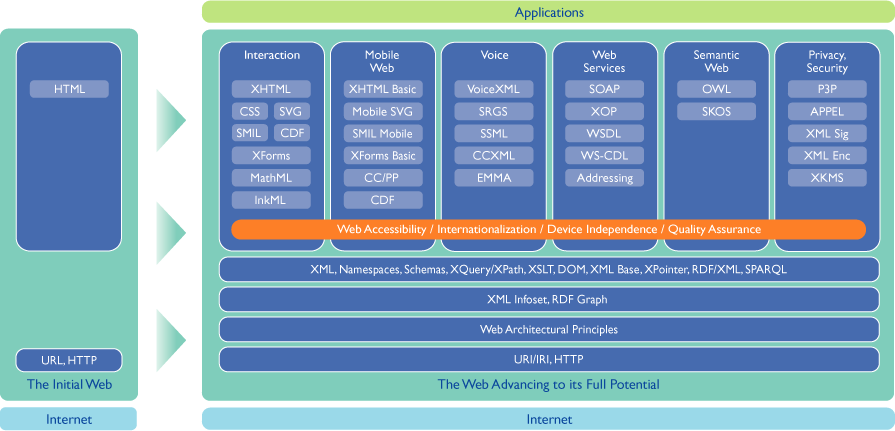
\includegraphics[width=12cm]{images/web-evolution.png}
	\caption{Evolución de la Web}
	\label{fig:evoWeb}
\end{figure}

En los últimos años la Web ha experimentado una notable evolución, como puede 
verse en la figura \ref{fig:evoWeb}\footnote{Fuente: W3C}, que le ha llevado a 
convertirse no sólo en un almacén de contenido estático, sino también en un 
repositorio universal de conocimiento y servicios.

A pesar de todas estas pequeñas revoluciones, todavía seguimos en una web 
\emph{sintáctica}. Hoy en día la llamada \emph{Web 2.0}\cite{O'Reilly2005} está
de actualidad, aunque todavía es una Web en la es muy difícil realizar muchas 
tareas que con la Web Semántica (\emph{¿Web 3.0?}), y todas sus tecnologías, 
al menos serán un poco más fácil de hacer.

\subsection{Estructura de la Web Semántica}

La Web Semántica se encuentra estructurada en capas (la llamada \emph{tarta de 
la Web Semántica}), de forma que se pudiera trabajar en cada uno de estos
sustratos de manera independiente a el estado de la implementación de las
capas inferiores y/o superiores.

Algunas parte del diseño aún se están discutiendo en los distintos grupos de
trabajo, aunque en la figura \ref{fig:swStack} encontramos el diseño que toma
más forma después de los últimos años de trabajo:

\begin{figure}[H]
	\centering
	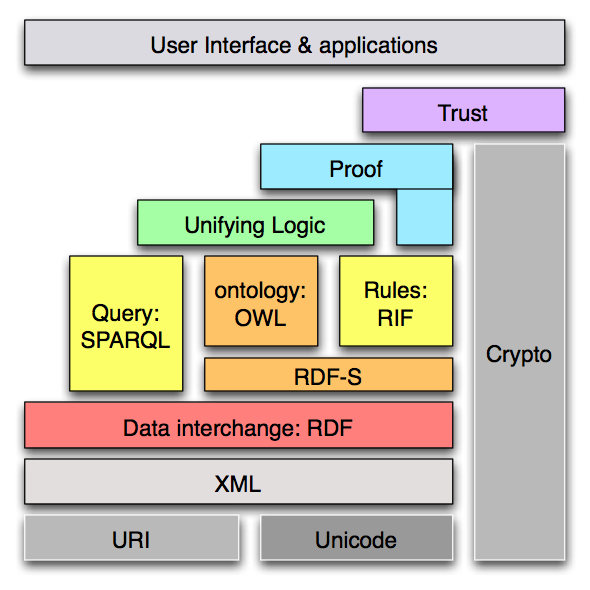
\includegraphics[width=10cm]{images/semantic-web-stack.png}
	\caption{Pila de la web semántica}
	\label{fig:swStack}
\end{figure}

Puede verse que el núcleo de la Web Semántica se construye sobre tres 
tecnologías fundamentales:

\begin{itemize}
  \item RDF\cite{Graham2004}
  \item OWL\cite{OWL}
  \item SPARQL\cite{Eric2006}
\end{itemize}

Con una envoltura de lógica y reglas, sustentadas sobre una infraestructura 
basada en XML, URI's y Unicode.

Véase que las reglas están a mismo nivel que las ontologías, y no por
encima como se pensaba en los primeros diseños, por la íntima relación que ambas
tienen.

\subsection{Elementos}

\subsubsection{Elementos básicos}

\paragraph{Unicode}es una iniciativa\footnote{\url{http://www.unicode.org/}} de 
un consorcio de empresas dedicadas a la internacionalización para conseguir una 
representación informática de los caracteres en todos los idiomas de forma que 
pueda ser representados y manipulados de forma universal. 

Aunque existen varias codificaciones distintas, UTF-8\cite{Yergeau2003} es la 
codificación unicode más usada y extendida, tanto por su sencillez (usa grupos 
de bytes) como por su flexibilidad (los alfabetos de muchos de los lenguajes 
del mundo se pueden representar en UTF-8).

Unicode es el recurso primario de representación de caracteres en la Web Semántica.

\paragraph{URI}acrónimo del inglés \emph{Uniform Resource Identifier}\cite{Berners-Lee1998}, 
identificador uniforme de recursos, es un mecanismo para la identificación de recursos
en red. Se trata de una especialización del IRI (Internationalized Resource Identifier) 
limitada al rango de caracteres ASCII.

Un concepto que mezcla URL\footnote{Uniform Resource Locator, localizador uniforme de recurso} 
y URN\footnote{Uniform Resource Name, nombre uniforme de recurso} para cumplir una doble 
funcionalidad: servir como protocolo de acceso e identificar de manera única los recursos 
en la World Wide Web.

\subsubsection{XML}

XML\cite{Bray2006} (eXtensible Markup Language\footnote{\url{http://www.w3.org/XML/}}, 
lenguaje  de marcado extensible) es un formato de marcado estructurado para la 
representación de información muy usado y extendido hoy en día, hasta tal punto de 
ser considerado el lenguaje universal para el intercambio de información. 

Desarrollado por el W3C a partir de SGML\footnote{\url{http://www.w3.org/MarkUp/SGML/}} 
con el objetivo que fuera fácilmente procesable por una máquina y legible por un 
humano. 

\begin{figure}[H]
\lstset{language=PeliculasXML}
\begin{lstlisting}
<?xml version="1.0" encoding="UTF-8"?>

<peliculas>

  <pelicula vista="true">
    <titulo>Resevoir Dogs</titulo>
    <autor>Quentin Tarantino</autor>
    <url>http://www.imdb.com/title/tt0105236/</url>
  </pelicula>

  <pelicula vista="false">
    ...
  </pelicula>

</peliculas>
\end{lstlisting}
\caption{Ejemplo de fichero en XML}
\label{fig:ejemplo.xml}
\end{figure}

Basándose en una definición abstracta (XML Schema\footnote{\url{http://www.w3.org/XML/Schema}}), 
permite extender su gramática de una forma muy fácil y sencilla de procesar 
(XSL/XSLT, XPath, XPointer, etc).

Es usado en múltiples tecnologías hoy en día, sobre todo en la web (XHTML, XForms, 
SVG, etc), aunque también para documentación (DocBook), interfaces de usuario (XUL,
Glade, XAML, etc), protocolos (Jabber), etc. Se utilizan espacios de nombres (namespace), 
identificados por URI's, para mezclar en un documento etiquetas pertenecientes a 
diferentes vocabularios.

Pero XML, a pesar de ser un lenguaje estructurado que es muy fácil de procesar, 
aún carece de la semántica necesaria. 

Sobre XML existe mucha bibliografía relacionada, siendo recomendable empezar por
\emph{XML Imprescindible}\cite{XMLNutshell}, un excelente libro que hace un amplio
recorrido por XML y todas sus tecnologías.

\subsubsection{RDF}

Acrónimo del inglés \emph{Resource Description Framework} (marco de descripción 
de recursos), RDF\footnote{\url{http://www.w3.org/RDF/}} es una especificación del 
W3C originalmente diseñada como modelo de metadatos, pero su uso se ha extendido como
método general para modelar el conocimiento.

RDF se basa en un modelo de tripletas del tipo \texttt{(sujeto, predicado, objeto)}. El
sujeto es un recurso que se identifica con una URI, y se relaciona mediante un 
predicado binario con el objeto, que puede ser otra URI o un literal.

\begin{figure}[H]
	\centering
	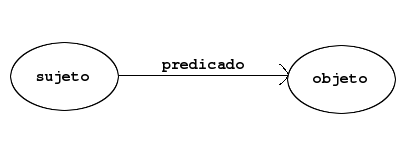
\includegraphics[width=10cm]{images/arc.png}
	\caption{Arco RDF}
	\label{fig:rdfTriplet}
\end{figure}

Cada tripleta puede verse como un arco, y al juntarse con otros arcos se obtiene
un grafo dirigido que describe los recursos y las relaciones entre todos los 
recursos.

Un ejemplo sencillo: \textit{Sergio Fdez es el creador de http://www.wikier.org/}. 
Usando Dublin Core (sección \ref{sec:dc}) podría quedar la siguiente tripleta: 
\texttt{(http://www.wikier.org/, dc:creator, "Sergio Fdez")}. Dando lugar a un 
grafo del estilo del que se puede ver en la figura~\ref{fig:rdfTripletExample}.

\begin{figure}[H]
	\centering
	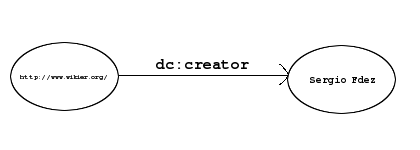
\includegraphics[width=12cm]{images/arc-example.png}
	\caption{Ejemplo de arco RDF}
	\label{fig:rdfTripletExample}
\end{figure}


RDF se puede serializar en tres sintaxis: 

\begin{itemize}
 \item XML\footnote{\url{http://www.w3.org/TR/rdf-syntax-grammar/}}
 \item N3\footnote{\url{http://www.w3.org/DesignIssues/Notation3}} (notación de tripletas)
 \item Turtle\footnote{\url{http://www.dajobe.org/2004/01/turtle/}}
\end{itemize}

El mismo grafo de la figura~\ref{fig:rdfTripletExample} se podría serializar 
con las tres sintaxis, conteniendo las tres representaciones idéntica información 
semántica:

\begin{figure}[H]
\lstset{language=RDF}
\begin{lstlisting}
<rdf:RDF xmlns:rdf="http://www.w3.org/1999/02/22-rdf-syntax-ns#"
         xmlns:rdfs="http://www.w3.org/2000/01/rdf-schema#"
         xmlns:dc="http://purl.org/dc/elements/1.1/"
>

  <rdf:Description rdf:about="http://www.wikier.org/">
    <dc:creator>Sergio Fdez</dc:creator>
  </rdf:Description>

</rdf:RDF>
\end{lstlisting}
\caption{Ejemplo de grafo RDF serializado en XML}
\label{fig:ejemplo.rdfxml}
\end{figure}

\begin{figure}[H]
\lstset{language=N3}
\begin{lstlisting}
@prefix dc <http://http://purl.org/dc/elements/1.1/>

<http://www.wikier.org> dc:creator "Sergio Fdez"
\end{lstlisting}
\caption{Ejemplo de grafo RDF serializado en N3}
\label{fig:ejemplo.rdfn3}
\end{figure}

\begin{figure}[H]
\lstset{language=Turtle}
\begin{lstlisting}
@prefix dc <http://http://purl.org/dc/elements/1.1/>

<http://www.wikier.org> 
	dc:creator "Sergio Fdez"
\end{lstlisting}
\caption{Ejemplo de grafo RDF serializado en Turtle}
\label{fig:ejemplo.rdfturtle}
\end{figure}

\subsubsection{RDFS}

RDFS (RDF Schema\cite{RDFS}) es una forma primitiva y limitada de describir 
ontologías en RDF, también llamado «\emph{vocabulario RDF}». Provee los elementos
básicos para la definición de ontologías (clases, subclases, propiedades, etc)
\footnote{¿Qué es una ontología? La mejor definición es la que da Tom Gruber
en \url{http://www-ksl.stanford.edu/kst/what-is-an-ontology.html}}.

Aunque OWL, del que hablaremos a continuación, es mucho más expresivo, aún muchas
ontologías se encuentras definidas con RDFS.

\subsubsection{OWL}

Acrónimo resultante de \emph{retorcer} el nombre de 
\emph{Web Ontology Language}, OWL\cite{OWL} es la recomendación 
oficial de W3C\footnote{\url{http://www.w3.org/}} para publicar ontologías en 
la Web. Se trata de un lenguaje de gran expresividad para describir conceptos 
y relaciones entre conceptos, con un compromiso entre expresividad y tratabilidad.

Es la versión revisada y mejorada de juntar dos lenguajes más viejos para la 
definición de ontologías como son DAML\footnote{\url{http://www.daml.org/}} y 
OIL\footnote{\url{http://www.ontoknowledge.org/oil/}} (lo llamado
DAML+OIL\footnote{\url{http://www.daml.org/2001/03/daml+oil-index}}).

La versión actual de OWL, la 1.0 (la 1.1 aún se encuentra en estos momentos en 
fase de desarrollo bajo el liderazgo del español Bernardo 
Cuenca\footnote{\url{http://www.cs.man.ac.uk/~bcg/}}), tiene 
tres variantes según su complejidad y expresividad:

\begin{itemize}
  \item \textbf{OWL Full}, íntimamente ligado a la lógica de RDF, pero que puede 
	resultar no computable.
  \item \textbf{OWL DL}, un subconjunto del anterior basado en la lógica 
	descriptiva ${SHOIN} (D)$.
  \item \textbf{OWL Lite}, subconjunto de OWL DL que se basa en la lógica 
	descriptiva de menor expresividad ${SHIF} (D)$.
\end{itemize}

Una perspectiva sencilla sería la mostrada por la figura~\ref{fig:owlVariants}.

\begin{figure}[H]
	\centering
	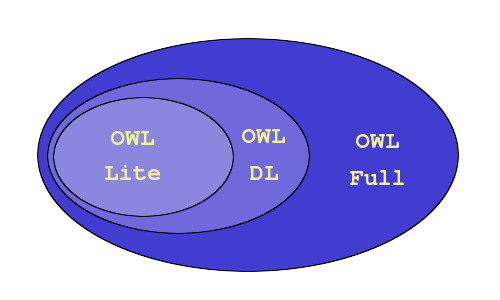
\includegraphics[width=12cm]{images/owl-variants.png}
	\caption{Perspectiva sencilla de OWL}
	\label{fig:owlVariants}
\end{figure}

Aunque el panorama no es tan sencillo, y para diferenciar cada una de ellas no
se puede hacer fijándose sólo en la complejidad, sino también en la parte de la 
lógica que abarcan. Quedando un panorama aún más confuso, como se puede ver en 
la figura \ref{fig:owlVariantsExtended}\footnote{Gráfico extraído de Ontotext, 
\url{http://www.ontotext.com/inference/rdfs_rules_owl.html#owl_fragments}}.

\begin{figure}[H]
	\centering
	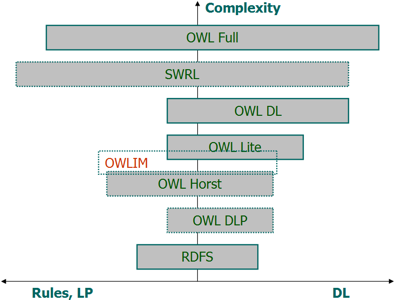
\includegraphics[width=10cm]{images/owl-dialects.png}
	\caption{Variantes de OWL ampliado}
	\label{fig:owlVariantsExtended}
\end{figure}

Hay que tener en cuenta que existe cierto solapamiento entre la expresividad de
OWL y la de RDFs (RDF-Schema), desvirtuando en cierta manera la visión original
por capas.

Para más información puede consultarse el último libro publicado acerca de 
OWL\cite{OWLBook}.

\subsubsection{SPARQL}

SPARQL\footnote{\url{http://www.w3.org/TR/rdf-sparql-query/}} es un nuevo lenguaje
de consulta sobre la base del conocimiento en OWL/RDF. No es el único\cite{ComparisonRDFQuery},
aunque si el más completo y la apuesta oficial del W3C en este área, debido a que es
un lenguaje con un compromiso en su justa medida entre semántica y 
complejidad\cite{SemanticsComplexitySPARQL}. 

Actualmente se trata del candidato a recomendación del W3C por parte del 
DAWG\footnote{\url{http://www.w3.org/2001/sw/DataAccess/}} (RDF Data Access Working 
Group).

Posee una sintaxis similar a la otros lenguajes de consulta relacionales, como
podría ser SQL. De hecho sus 
álgebras\footnote{\url{http://www.w3.org/2001/sw/DataAccess/rq23/rq24-algebra.html}} comparten\cite{RelationalAlgebraSPARQL} determinados puntos. 

\begin{figure}[H]
\lstset{language=SPARQL}
\begin{lstlisting}
PREFIX rdf: <http://www.w3.org/1999/02/22-rdf-syntax-ns#>
PREFIX dc: <http://purl.org/dc/elements/1.1/>

SELECT DISTINCT ?x, ?name
WHERE {
	?x dc:creator ?name
}
\end{lstlisting}
\caption{Ejemplo de consulta SPARQL}
\label{fig:ejemplo.sparql}
\end{figure}

Aplicando esta sencilla consulta de ejemplo a un RDF, como por ejemplo el de 
antes \ref{fig:ejemplo.rdfxml}, se obtendría el nombre del creador de cada recurso
definido.

A pesar de ser un lenguaje relativamente reciente, ya se encuentran disponibles
API's de consulta para numerosos lenguajes de programación: 
RDFLib\footnote{\url{http://rdflib.net/sparql/}} para Python, 
Jena\footnote{\url{http://jena.sourceforge.net/ARQ/}} en Java, 
Redland RDF\footnote{\url{http://librdf.org/}} en C con bindings también para 
otros lenguajes, twinql\footnote{\url{http://www.holygoat.co.uk/projects/twinql/}} 
en Lisp, etc. Además de estar soportado por alguno de los razonadores\footnote{Un 
razonador es un componente software que permite operar lógicamente sobre una base 
de conocimiento, por ejemplo para verificar su consistencia o inferir nueva
información.} más conocidos, como Pellet\footnote{\url{http://www.mindswap.org/2003/pellet/}} 
o KAON2\footnote{\url{http://kaon2.semanticweb.org/}}.

\subsection{Aplicaciones prácticas}

\subsubsection{Vocabularios RDF}

Existen multitud de vocabularios RDF para fines muy concretos, desde describir
personas, hasta eventos. Estos vocabularios suelen ser fácilmente extensibles y 
reutilizables entre si.

Existen multitud de ejemplos:

\begin{itemize}
  \item \textbf{Dublin Core\label{sec:dc}:} Dublin Core\footnote{\url{http://dublincore.org/}}, 
	también conocido por sus siglas \texttt{DC}, es un vocabulario RDF para la descripción 
	de múltiples propiedades de todo tipo de recursos online.

	Por ejemplo se ha usado Dublin Core en el ejemplo descrito en la 
	figura~\ref{fig:rdfTripletExample}, y evidentemente también en sus distintas 
	serializaciones (figura~\ref{fig:ejemplo.rdfxml}, figura~\ref{fig:ejemplo.rdfn3} 
	y figura~\ref{fig:ejemplo.rdfturtle}).

  \item \textbf{RSS:} Desarrollado en el seno de Netscape, RSS es el formato de sindicación de 
	noticias más extendido en la actualidad. Con un complicado historial, como se puede ver 
	en la figura~\ref{fig:rssEvolution}, de versiones incompatibles entre sí; de hecho sólo 
	la versión 1.0 de RSS es RDF, el resto de versiones han introducido ciertos aspectos
	incompatibles.

	\begin{figure}[H]
		\centering
		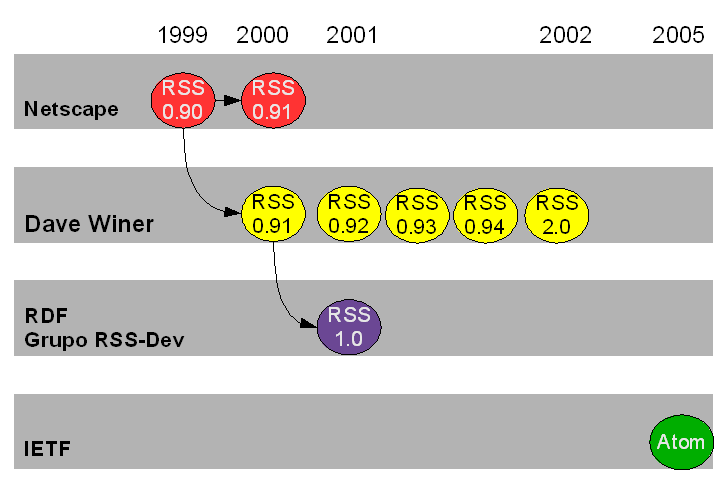
\includegraphics[width=10cm]{images/rssEvolution.png}
		\caption{Evolución de RSS}
		\label{fig:rssEvolution}
	\end{figure}

  \item \textbf{FOAF:} FOAF\footnote{\url{http://www.foaf-project.org/}}, acrónimo de 
	\emph{Friend-of-a-Friend}, se trata de un vocabulario RDF para describir 
	semánticamente información personal muy extendido (en 2004 se estimaba\cite{Li2005} 
	que existían alrededor de 1,2 millones de documentos FOAF) dentro del ámbito 
	de la web semántica.

\begin{figure} [H]
\lstset{language=RDF}
\begin{lstlisting}
<rdf:RDF
	xmlns:rdf="http://www.w3.org/1999/02/22-rdf-syntax-ns#"
	xmlns:rdfs="http://www.w3.org/2000/01/rdf-schema#"
	xmlns:foaf="http://xmlns.com/foaf/0.1/"
>

  <foaf:Person rdf:about="http://www.wikier.org/foaf.rdf#wikier">
    <foaf:name>Sergio Fdez</foaf:name>
    <foaf:title>Mr</foaf:title>
    <foaf:firstName>Sergio</foaf:firstName>
    <foaf:surname>Fdez</foaf:surname>
    <foaf:gender>Male</foaf:gender>
    <foaf:mbox>sergio@wikier.org</foaf:mbox>
  </foaf:Person>

</rdf:RDF>
\end{lstlisting}
\caption{Ejemplo de FOAF}
\label{fig:ejemplo.foaf}
\end{figure}

	Pudiendo describir relaciones (amigos, compañeros de trabajo, etc), intereses,
	proyectos y demás recursos de uso personal, de forma que se forme un grafo 
	uniendo todos ellos. El patrón\ref{fig:patternFOAF} siempre se repite.

	\begin{figure}[H]
		\centering
		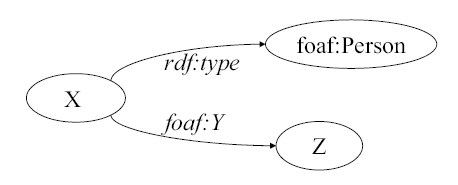
\includegraphics[width=7cm]{images/patron-foaf.png}
		\caption{Patrón de documentos FOAF}
		\label{fig:patternFOAF}
	\end{figure}

  \item \textbf{DOAP:} \emph{Description-of-a-Project\footnote{\url{http://usefulinc.com/doap}}} 
	es una idea similar a FOAF pero para describir todo tipo de proyectos.

\begin{figure}[H]
\lstset{language=RDF}
\begin{lstlisting}
<rdf:RDF xmlns:rdf="http://www.w3.org/1999/02/22-rdf-syntax-ns#" 
         xmlns:rdfs="http://www.w3.org/2000/01/rdf-schema#" 
         xmlns:doap="http://usefulinc.com/ns/doap#" 
         xmlns:foaf="http://xmlns.com/foaf/0.1/" 
         xmlns:admin="http://webns.net/mvcb/" 
>

  <doap:Project rdf:about="http://swaml.berlios.de/">

    <doap:name>Semantic Web Archive of Mailing Lists</doap:name>
    <doap:shortname>SWAML</doap:shortname>

    <doap:description>
      SWAML is a research project around the semantic web tecnologies 
      to publish the mailing lists archive into a RDF format.
    </doap:description>

    <doap:homepage rdf:resource="http://swaml.berlios.de/" />
    <doap:wiki rdf:resource="http://swaml.berlios.de/wiki" />
    <doap:license rdf:resource="http://usefulinc.com/doap/licenses/gpl" />

  </doap:Project>

</rdf:RDF>
\end{lstlisting}
\caption{Fichero DOAP de SWAML}
\label{fig:ejemplo.doap}
\end{figure}

  \item \textbf{EARL:} EARL\cite{EARL} (\emph{Evaluation and Report Language}, 
	en español \emph{Lenguaje de Evaluación de informes} es un vocabulario 
     	RDF para la grabación, transferencia y procesamiento de datos sobre 
	evaluaciones automáticas. Es usado por ejemplo por algunas herramientas
	de validación automática de la accesibilidad Web, como el
	TAW\footnote{\url{http://www.tawdis.net/}}, para expresar el
	resultado de sus evaluaciones.

\end{itemize}

\subsubsection{Otras aplicaciones de RDF}

\begin{itemize}
  \item \textbf{Framework Mozilla:} Firefox utiliza RDF internamente para 
	describir muchos aspectos del navegador. Por ejemplo un fichero como 
	el mostrado en la figura~\ref{fig:rdf.firefox} se utiliza en sus
	extensiones para describirlas semánticamente.

\begin{figure}[H]
\lstset{language=RDF}
\begin{lstlisting}
<?xml version="1.0" encoding="utf-8"?>

<rdf:RDF 
	xmlns:rdf="http://www.w3.org/1999/02/22-rdf-syntax-ns#"
	xmlns:em="http://www.mozilla.org/2004/em-rdf#"
>

  <rdf:Description rdf:about="urn:mozilla:install-manifest">
    <em:creator>Sergio Fdez</em:creator>
    <em:description>
      FOAFox, discover FOAF profiles in Firefox
    </em:description>
    <em:homepageURL>
      http://www.wikier.org/archivos/firefox/foafox/
    </em:homepageURL>
    <em:id>{5be0dd31-4194-4543-b29c-72248db06b71}</em:id>
    <em:name>FOAFox</em:name>
    <em:iconURL>chrome://foafox/skin/foafox.png</em:iconURL>
    <em:updateURL>
      http://www.wikier.org/archivos/mozilla/foafox/update.rdf
    </em:updateURL>
    <em:version>0.2.1</em:version>
    <em:targetApplication>
      <rdf:Description>
        <em:id>{ec8030f7-c20a-464f-9b0e-13a3a9e97384}</em:id>
        <em:minVersion>1.5</em:minVersion>
        <em:maxVersion>2.0.0.*</em:maxVersion>
      </rdf:Description>
    </em:targetApplication>
  </rdf:Description>

</rdf:RDF>
\end{lstlisting}
\caption{Ejemplo fichero RDF para describir una extensión de Mozilla Firefox}
\label{fig:rdf.firefox}
\end{figure}

\end{itemize}


\subsection{Futuro}

Hacia donde irá la Web Semántica es algo que sólo se sabrá con el tiempo, y quizás
en un plazo no más allá de 5 o 10 años. Por ahora es muy pronto para aventurar nada,
aunque si bien es cierto que el estado de adopción de la Web Semántica, en palabras
del propio Ivan Herman\footnote{\url{http://www.w3.org/2006/Talks/1109-Athens-IH/}}
(líder de la actividad de web semántica del W3C), crece a un ritmo imparable.

Históricamente han existido áreas de investigación vendidas en exceso como la 
panacea de la solución de todos los problemas de la humanidad; generando unas 
expectativas falsas que han hecho mucho daño a la comunidad científica.

Lo que si sabemos es que la Web Semántica será una Web mucho más \emph{útil}.





\chapter{Metodolog�a}

Las circunstacias profesionales del alumno en el periodo que se realiz� el
proyecto hicieron que se tomaran de forma natural muchos de los m�todos de
las metodolog�as �giles, de manera que permitiera un �ptimo y flexible reparto 
de tiempos entre todas las tareas a desarrollar a lo largo del proyecto.

As� se termin� utilizando de manera natural muchas de las normas de este tipo
de m�todos:

\begin{itemize}
  \item Simplicidad: desde el primer momentos se busc� hacer el proyecto de la 
	manera m�s sencilla posible.
  \item Desarrollo iterativo e incremental: una vez se fue teniendo las 
	funcionalidades principales, construyendo alrededor de los casos de uso
	principales peque�as utilidades para enriquecer la aplicaci�n.
  \item Propiedad del c�digo compartida: desde las primeras lineas, todo el 
	c�digo ha estado publicado en el 
	Subversion\footnote{\url{http://subversion.tigris.org/}}  del proyecto, 
	al alcance en cualquier momento de las tres personas involucradas en el 
	proyecto.
  \item Refactorizaci�n del c�digo: de manera frecuente partes del c�digo del 
	proyecto han sido sometidas a t�cnicas de refactorizaci�n para mejorar 
	partes que no hab�a sido codificadas de la mejor de las maneras.
  \item Pruebas unitarias (FIXME: mentira, pero es una tarea que tengo que abordar 
	con PyUnit)
  \item Frecuente interacci�n del equipo de programaci�n con el cliente o usuario:
	en este caso la figura del cliente ha tenido la forma del co-director del
	proyecto (Diego Berrueta), con el que se han mantenido frecuentes encuentros
	para tratar aspectos concretos del proyecto.
\end{itemize}




\chapter{Manuales}

En esta documentación se incluyen tres manuales:

\begin{itemize}
  \item Manual técnico (incluye el código fuente en un anexo).
  \item Manual de despliegue
  \item Manual de usuario.
\end{itemize}

\section{Manual técnico}

FIXME(contar como continuar con el proyecto)

\section{Manual de despliegue}

FIXME(contar como desplegar swaml)

\subsection*{Requisitos técnicos}

FIXME

\subsubsection{Interprete de Python}

Python (>=2.4), IronPython u otros...

\subsubsection{Bibliotecas necesarias}

Como se puede ver en la sección \ref{sec:conclu:bib}, han sido varias las
bibliotecas utilizadas en el proyecto.

FIXME

\begin{itemize}
  \item RDFLib
  \item dom.xml
\end{itemize}

\section{Manual de usuario}

FIXME(como usar swaml)



\chapter{Conclusiones}

FIXME

\section{Conclusiones personales}

Este proyecto me ha supuesto muchas cosas a nivel personal y profesional. He
aprendido mucho sobre esta incipiente área que es la Web Semántica; tengo la
suerte de contar con dos directores de proyecto (José Emilio Labra y Diego
Berrueta) que grandes expertos en la materia y me han ayudado en todos estos
meses.

Además me ha brindado la oportunidad de un nuevo lenguaje de programación al
que hacia tiempo le tenía ganas: Python.

Desde el punto de vista ético para mi era muy importante saber que las horas
invertidas en este proyecto no se \emph{morirían} en las polvorientas estanterias
de la biblioteca. Por eso desde eso desde el principio y en todo momento el
proceso de desarrollo de todos los componentes de este proyecto ha estado
disponible en el subversion de Berlios\footnote{\url{http://swaml.berlios.de/wsvn}}.

En estos meses he liberado media docena de versiones de SWAML. Quizás el recorrido
termine aquí, o quizás no. No sé si yo continuaré desarrollando SWAML o si a alguien
le parecerá interesante para continuar el trabajo que yo he comenzado; pero el caso
es que el software liberado ahí seguirá para cualquiera que sea el uso que alguien
le quiera dar.

\section{Conclusiones sobre la aportación de SWAML}

FIXME(SIOC, etc)

\section{Trabajo relacionado}

FIXME(¿la idea de swaml a que más podría aplicarse?)

\section{Conclusiones sobre el software utilizado}

Ha sido mucha la diversidad de software (complidores, bibliotecas y herramientas)
utilizado para la realización de este proyecto. Nótese que todo él se ha podido
desarrollar utilizando únicamente \emph{software libre}.

\subsection{Python}

FIXME

\subsection{Bibliotecas\label{sec:conclu:bib}}

FIXME(¿más?)

\subsubsection{RDFLib}

RDFLib\footnote{\url{http://rdflib.net/}} FIXME

\subsubsection{dom.xml}

dom.xml\footnote{\url{http://docs.python.org/lib/module-xml.dom.html}} FIXME

\subsubsection{PyGTK}

FIXME

\subsection{Herramientas}

FIXME

\subsubsection{Subversion}

Se han hecho 458 commits (FIXME: actualizar antes de imprimir)

\begin{figure}[ht]
	\centering
	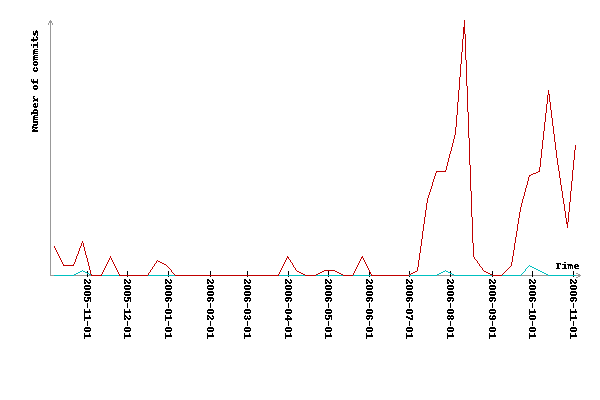
\includegraphics[width=15cm]{images/svn-stats.png}
	\caption{Estadísticas del subverion de SWAML}
	\label{fig:svnStats}
\end{figure}

\subsubsection{Autotools}

FIXME

\subsubsection{PyDev}

PyDev es un plugin para Eclipse FIXME

\subsubsection{Ant}

FIXME

\subsubsection{Gazpacho}

FIXME

\subsubsection{SWOOP}

Existen varios editores libres para ontologías OWL:

\begin{itemize}
  \item Protégé\footnote{\url{http://protege.stanford.edu/plugins/owl/}}
  \item SWeDE\footnote{\url{http://owl-eclipse.projects.semwebcentral.org/}}
  \item SWOOP\footnote{\url{http://www.mindswap.org/2004/SWOOP/}}
\end{itemize}

Los dos primeros no son más que plug-ins para dar soporte a OWL en dos 
frameworks. Y el tercero es un editor pensado y desarrollado explicitamente
para trabajar con OWL.

Después de las pruebas realizadas, SWOOP resultó ser una herramienta más sencilla,
comoda de usar y potente que las otras dos.

\begin{figure}[ht]
	\centering
	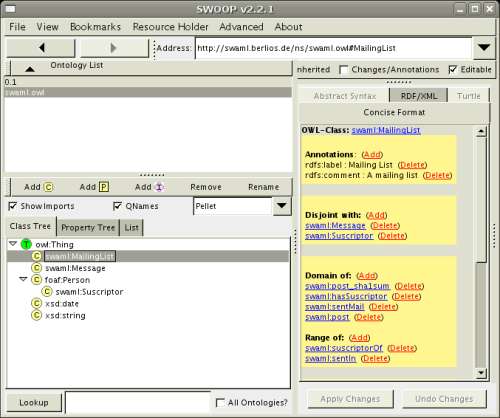
\includegraphics[width=11cm]{images/swoop.png}
	\caption{SWOOP editando la ontología de SWAML en OWL DL}
	\label{fig:evoWeb}
\end{figure}

Alguna de las caracteristicas más interesantes de SWOOP son:

\begin{itemize}
  \item Interfaz de usuario hypermedia similar a la de un navegador convencional, 
	con elementos (pestañas, marcadores, etc) que hacen la interfaz más 
	amigable.
  \item Soporte de depuración de la ontología.
  \item Cliente para hacer razonamientos sencillos con Pellet.
  \item FIXME
\end{itemize}

Un problema común en todas estas herramientas de alto nivel para trabajar con
grafos RDF es el serializado del grafo a sintáxis XML. No por su corrección,
que la herramienta lo hace perfectamente, sino por su orden: es muy difícil
que al serializar queden todos los nodos en el mismo orden. Por tanto es muy
difícil conocer las diferencias entre distintas versiones con las herramientas
convencionales (principalmente \texttt{diff}).

\subsubsection{phpWiki}

FIXME

\subsubsection{Google Maps}

FIXME(KML)

\subsubsection{\LaTeX}

\TeX/\LaTeX FIXME

\paragraph{Kile}

\paragraph{JabRef}

\section{Lineas de futuro}

El trabajo realizado hasta ahora con SWAML no ha hecho sino empezar, abriendo las 
puertas hacia una linea de desarrollo que puede significar un foco importante
en cuanto a la publicación en formatos semánticos de todo el conocimiento contenido
en esas miles de listas de correo existentes por lo largo y ancho de la internet
actual.

Aunque puede que no se incluyan todas las existentes, estas on algunas de las lineas
que seria interesante el proyecto abarcara algún día:

\subsection*{Integración con Mailman}

FIXME

\subsection*{API para DIG}

Sería interesante disponer de una API en Python para utilizar razonadores DL que implementen 
el protocolo DIG\footnote{\url{http://dig.cs.manchester.ac.uk/}}. 

Existen ya API's similares en Java (dentro del framework
Jena\footnote{\url{http://jena.sourceforge.net/how-to/dig-reasoner.html}} o incluso en Haskell 
(implementada dentro del proyecto WESO\footnote{\url{http://weso.sourceforge.net/}}. Por eso 
sería interesante implementar el protocolo DIG en Python, y no sería una tarea
en la que nos encontraríamos en solitario\cite{PythonOWL}.

FIXME



\appendix



\chapter{Propuesta inicial\label{sec:propuesta}}

Diego Berrueta (Agosto 2005)

Las listas de correo son parte fundamental de la comunicación en Internet.
Existen listas de correo dedicadas a cualquier tema de inter\'es imaginable.
Hoy en día, es común que las listas de correo publiquen sus archivos (los
mensajes antiguos) en forma de páginas web, lo que dispara su utilidad,
especialmente en combinación con los buscadores actuales. Gracias a esta 
publicación, es posible consultar los mensajes desde el navegador, sin 
necesidad de estar suscrito a las listas de correo, y también se puede 
localizar un mensaje usando Google u otro buscador.

Estos archivos contienen una formidable base de conocimiento, especialmente
en temas técnicos. Un uso muy común consiste en introducir un mensaje de error 
(de una aplicación) en Google\footnote{\url{http://www.google.es/}} y obtener 
como resultado un mensaje archivado que aborda el problema, probablemente 
porque alguien se ha encontrado previamente con el mismo error y ha efectuado 
la consulta en una lista de correo pública. Con suerte, alguna de las respuestas 
al mensaje localizado contendrá la solución al problema, aportada por un experto 
suscrito a la lista de correo.

\section*{Problemas}

Por desgracia, consultar los archivos de una lista de correo en la web es
más incómodo que hacerlo mediante un cliente de correo electrónico.
Por poner sólo algunos ejemplos, el navegador no permite ejecutar ninguna
de estas acciones:

\begin{itemize}
 \item Mostrar el hilo de la conversación en forma de árbol.
 \item Imprimir el hilo completo.
 \item Mostrar una lista de los mensajes entre dos fechas arbitrarias.
 \item Ocultar los mensajes que no tienen respuestas.
 \item Mostrar sólo los mensajes de una cierta persona.
 \item Buscar una cadena de texto sólo en los mensajes de un determinado hilo.
 \item Descargar el hilo como un fichero, o cualquier otra forma de exportar la
 información para poder acceder a ella desde un cliente de correo electrónico
 o fuera de línea.
 \item Responder a un mensaje usando un cliente de correo (o un webmail) y 
 citando el mensaje original.
\end{itemize}

Al indexar los archivos de las listas de correo, los buscadores se encuentran
en ocasiones que los mensajes están replicados en varios servidores (mirrors).
Al no tener forma de identificar los mensajes, la desgraciada consecuencia
es que los mensajes aparecen varias veces en los resultados de las búsquedas,
y sólo el usuario puede darse cuenta de que se trata de una repetición.
Naturalmente, el comportamiento ideal sería que los mensajes aparecieran
sólo una vez en los resultados del buscador.

\section*{Origen de los problemas: pérdida de información}

En el origen de estos problemas se encuentra una pérdida de información
que se produce al convertir los mensajes archivados a HTML para su publicación
en la web.

Los gestores más habituales de listas de correo (mailman, majordomo, sympa,
etc.) generan un fichero en formato Mailbox (mbox) con los mensajes que
han sido enviados a la lista.

Otros programas independientes, como hypermail, monharc, pipermail..., se
especializan en convertir el fichero Mailbox en un conjunto de páginas
web estáticas.

Los programas más sofisticados son capaces de generar índices complejos
de los archivos (por fecha, por autor, por hilo...), con múltiples referencias
cruzadas entre los mensajes en forma de hipervínculos (mensaje anterior,
mensaje siguiente, etc.).

Pero incluso en el mejor de los casos, esta información sólo es comprensible
para el usuario, nunca para la máquina.

En consecuencia, es imposible explotarla más allá de las formas previstas
por el programa que ha generado los archivos.

Entre la información que se pierde en la publicación, se encuentra:

\begin{itemize}
 \item El asunto del mensaje.
 \item El autor del mensaje.
 \item La fecha del mensaje.
 \item La referencia a la lista de correo en la que se publicó el mensaje.
 \item La referencia al mensaje anterior, si existe.
 \item Las referencias (enlaces) a las posibles respuestas al mensaje.
\end{itemize}

\section*{Propuesta para conservar la información}

Las tecnologías de la web semántica (y concretamente, RDF) son perfectamente
capaces de publicar en la web toda la información señalada en la sección
anterior. Dado que la información ya existe en el origen, no es necesario 
ningún procedimiento manual para enriquecerla. Tan sólo debe considerarse un 
proceso de conversión que no desprecie la información, sino que la publique 
junto con los archivos en HTML. De esta forma, las listas de correo se 
introducirían en la web semántica.

\section*{Aplicaciones}

Enriquecer semánticamente la publicación web de los archivos de las listas
de correo abriría la puerta a nuevas aplicaciones:

\begin{itemize}
  \item Eliminar la aparición repetida de los mismos mensajes en los resultados
 	de los buscadores. Para lograrlo, los buscadores deberían procesar la 
	información semántica para reconocer las copias (mirrors) de los archivos.
  \item Implementar en los navegadores nuevas funcionalidades para resolver alguno
	de los problemas antes señalados. Estas capacidades, que mejorarían 
	sensiblemente la comodidad en la consulta de los archivos, podrían añadirse 
	como extensiones o plug-ins de los navegadores actuales.
  \item Obtener información sobre los suscriptores de una lista de correo. Por 
	ejemplo, conocer en qué otras listas de correo participa una persona. 
	Esta aplicación es especialmente interesante en conexión con 
	FOAF\footnote{\url{http://www.foaf-project.org/}.} De este modo, se 
	podría sacar una \emph{orla} con las fotos de los participantes en una 
	lista de correo\footnote{Como hace GNOME, véase 
	\url{http://planet.gnome.org/heads/}}, o situarlos geográficamente en un 
	mapa\footnote{Como hace Debian, 
	véase \url{http://www.debian.org/devel/developers.loc}}.
  \item Facilitar la internacionalización. Al hacer comprensibles las relaciones entre 
	los mensajes por el software, el navegador proporcionaría las opciones de 
	exploración (mensaje siguiente, mensaje anterior, etc.) en el idioma del 
	usuario, independientemente del idioma en el que se encontrasen las páginas 
	HTML.
  \item Mejorar la accesibilidad de la información. Las tecnologías de accesibilidad 
	podrían informar sobre quién es el autor del mensaje o cuántas respuestas hay, 
	usando la voz u otros medios.
\end{itemize}

\section*{Estado del arte}

Existen algunos trabajos similares a esta propuesta:

\begin{itemize}
  \item El proyecto DOAML\footnote{\url{http://www.doaml.net/}} consiste en un 
	vocabulario RDF para describir listas de correo. Como ejemplo, en 
	la web del proyecto se encuentran las descripciones de las listas 
	de correo del W3C. La información de este vocabulario limita sus 
	referencias a los mensajes archivados a un enlace a la versión HTML 
	de éstos.
  \item Por otro lado, EMiR\footnote{\url{http://xmlns.filsa.org/emir/}} es un 
	esquema RDF para describir mensajes de correo electrónico. 
  \item En la misma línea se encuentra XMTP\footnote{\url{http://www.openhealth.org/xmtp/}}.
\end{itemize}

\section*{Conclusiones}

Introducir los archivos de las listas de correo en la web semántica sólo
requiere disponer de una aplicación de publicación que utilice la tecnología
apropiada (RDF) como complemento al HTML.

Con un mínimo esfuerzo, los administradores de todas las listas de correo
podrían emplear la aplicación en sus listas, por lo que la implantación
sería rápida\footnote{En realidad, cualquier suscriptor (no necesariamente 
el administrador) de una lista de correo podría publicar los archivos enriquecidos.
Tan sólo debería disponer de todos los mensajes antiguos almacenados en su 
cliente de correo electrónico, y exportarlos al formato Mbox.}. Además, al 
no requerirse la participación de un experto para el enriquecimiento de la 
información, resultaría posible enriquecer inmediatamente grandes volúmenes 
de información, incluso listas de correo que lleven muchos años en funcionamiento.

El desarrollo de una aplicación de estas características requeriría, en
primer lugar, la creación de un esquema de información, que muy bien podría
ser una combinación de los ya existentes; y en segundo lugar, el procesamiento 
de un fichero Mbox para extraer la información que contiene.



\chapter{Ontología}

Se ha desarrollado una sencilla ontología que formalizara las representación de 
una lista de correo que SWAML publica en RDF. 

\section{Version 0.1}\label{sec:ont:0.1}

La primera versión de la ontología modelaba una lista de correo con clases propias,
apoyandose únicamente en algunas clases y propiedades de 
FOAF\footnote{\url{http://www.foaf-project.org/}} y 
Dublin Core\footnote{\url{http://dublincore.org/}}.

La ontología definía tres clases para representar una lista de correo, relacionadas
como se puede ver en la figura~\ref{fig:swamlOWL}:

\begin{figure}[H]
	\centering
	\includegraphics[width=12cm]{images/swaml-owl.png}
	\caption{Representación gráfica de las clases principales descritas en la version 0.1 de la ontología de SWAML}
	\label{fig:swamlOWL}
\end{figure}

Además de las propiedades mostradas en la figura~\ref{fig:swamlOWL}, la ontología
definia otras muchas con rango a tipos de datos simples de
XMLSchema\footnote{\url{http://www.w3.org/2001/XMLSchema}}.

Esta versión 0.1 estaba desarrollada en OWL DL, disponiendo evidentemente
de una URI: \url{http://swaml.berlios.de/ns/01}.

\newpage

\lstset{language=XML}
\begin{lstlisting}
<?xml version="1.0"?>

<!DOCTYPE owl [
	<!ENTITY foaf "http://xmlns.com/foaf/0.1/">
	<!ENTITY dc "http://purl.org/dc/elements/1.1/">
	<!ENTITY xsd "http://www.w3.org/2001/XMLSchema#">
	<!ENTITY rdf "http://www.w3.org/1999/02/22-rdf-syntax-ns#">
	<!ENTITY owl "http://www.w3.org/2002/07/owl#">
	<!ENTITY rdfs "http://www.w3.org/2000/01/rdf-schema#">
	<!ENTITY swaml "http://swaml.berlios.de/ns/0.1#">
]>

<rdf:RDF
	xmlns:foaf="http://xmlns.com/foaf/0.1/"
	xmlns:dc="http://purl.org/dc/elements/1.1/"
	xmlns:xsd="http://www.w3.org/2001/XMLSchema#"
	xmlns:rdf="http://www.w3.org/1999/02/22-rdf-syntax-ns#"
	xmlns:owl="http://www.w3.org/2002/07/owl#"
	xmlns:rdfs="http://www.w3.org/2000/01/rdf-schema#"
	xmlns:swaml="http://swaml.berlios.de/ns/0.1#"
	xml:base="http://swaml.berlios.de/ns/0.1"
>

<owl:Ontology rdf:about="http://swaml.berlios.de/ns/0.1">
  <rdfs:comment>Ontology to describe mail lists</rdfs:comment>
  <owl:versionInfo>0.1</owl:versionInfo>
  <rdfs:label>SWAML Ontology</rdfs:label>
</owl:Ontology>

<owl:Class rdf:about="http://swaml.berlios.de/ns/0.1#MailingList">
  <rdfs:comment>A mailing list</rdfs:comment>
  <rdfs:label>Mailing List</rdfs:label>
  <owl:disjointWith>
    <owl:Class rdf:about="http://swaml.berlios.de/ns/0.1#Message">
    </owl:Class>
  </owl:disjointWith>
  <owl:disjointWith>
    <owl:Class rdf:about="http://xmlns.com/foaf/0.1/Person">
    </owl:Class>
  </owl:disjointWith>
</owl:Class>
<owl:Class rdf:about="http://swaml.berlios.de/ns/0.1#Message">
  <rdfs:label>Message</rdfs:label>
  <rdfs:comment>A mailing list message</rdfs:comment>
  <owl:disjointWith>
    <owl:Class rdf:about="http://xmlns.com/foaf/0.1/Person">
    </owl:Class>
  </owl:disjointWith>
</owl:Class>
<owl:Class rdf:about="http://swaml.berlios.de/ns/0.1#Suscriptor">
  <rdfs:subClassOf>
    <owl:Class rdf:about="http://xmlns.com/foaf/0.1/Person">
    </owl:Class>
  </rdfs:subClassOf>
  <rdfs:label>Suscriptor</rdfs:label>
  <rdfs:comment>A mailing list suscriptor</rdfs:comment>
</owl:Class>
<owl:Class rdf:about="http://www.w3.org/2002/07/owl#Thing">
</owl:Class>
<owl:Class rdf:about="http://xmlns.com/foaf/0.1/Person">
</owl:Class>

<owl:ObjectProperty rdf:about="http://swaml.berlios.de/ns/0.1#author">
  <rdfs:domain>
    <owl:Class rdf:about="http://swaml.berlios.de/ns/0.1#Suscriptor">
    </owl:Class>
  </rdfs:domain>
  <rdfs:range>
    <owl:Class rdf:about="http://swaml.berlios.de/ns/0.1#Message">
    </owl:Class>
  </rdfs:range>
  <owl:inverseOf rdf:resource="http://swaml.berlios.de/ns/0.1#from" />
  <rdfs:label>author</rdfs:label>
  <rdfs:comment>A person is the author of a message</rdfs:comment>
</owl:ObjectProperty>
<owl:ObjectProperty rdf:about="http://swaml.berlios.de/ns/0.1#from">
  <rdfs:domain>
    <owl:Class rdf:about="http://swaml.berlios.de/ns/0.1#Message">
    </owl:Class>
  </rdfs:domain>
  <rdfs:range>
    <owl:Class rdf:about="http://swaml.berlios.de/ns/0.1#Suscriptor">
    </owl:Class>
  </rdfs:range>
  <owl:inverseOf rdf:resource="http://swaml.berlios.de/ns/0.1#author" />
  <rdfs:label>from</rdfs:label>
  <rdfs:comment>A message was sent by a person</rdfs:comment>
</owl:ObjectProperty>
<owl:ObjectProperty rdf:about="http://swaml.berlios.de/ns/0.1#hasSuscriptor">
  <rdfs:domain>
    <owl:Class rdf:about="http://swaml.berlios.de/ns/0.1#MailingList">
    </owl:Class>
  </rdfs:domain>
  <rdfs:range>
    <owl:Class rdf:about="http://swaml.berlios.de/ns/0.1#Suscriptor">
    </owl:Class>
  </rdfs:range>
  <owl:inverseOf rdf:resource="http://swaml.berlios.de/ns/0.1#suscriptorOf" />
  <rdfs:label>hasSuscriptor</rdfs:label>
  <rdfs:comment>A mailing list has a suscriptor</rdfs:comment>
</owl:ObjectProperty>
<owl:ObjectProperty rdf:about="http://swaml.berlios.de/ns/0.1#nextByDate">
  <rdfs:domain>
    <owl:Class rdf:about="http://swaml.berlios.de/ns/0.1#Message">
    </owl:Class>
  </rdfs:domain>
  <rdfs:range>
    <owl:Class rdf:about="http://swaml.berlios.de/ns/0.1#Message">
    </owl:Class>
  </rdfs:range>
  <owl:inverseOf rdf:resource="http://swaml.berlios.de/ns/0.1#previousByDate" />
  <rdfs:comment>Next message sent in mailing list</rdfs:comment>
</owl:ObjectProperty>
<owl:ObjectProperty rdf:about="http://swaml.berlios.de/ns/0.1#previousByDate">
  <rdfs:domain>
    <owl:Class rdf:about="http://swaml.berlios.de/ns/0.1#Message">
    </owl:Class>
  </rdfs:domain>
  <rdfs:range>
    <owl:Class rdf:about="http://swaml.berlios.de/ns/0.1#Message">
    </owl:Class>
  </rdfs:range>
  <owl:inverseOf rdf:resource="http://swaml.berlios.de/ns/0.1#nextByDate" />
  <rdfs:comment>Previous message by date in mailign list</rdfs:comment>
  <rdfs:label>previousByDate</rdfs:label>
</owl:ObjectProperty>
<owl:ObjectProperty rdf:about="http://swaml.berlios.de/ns/0.1#sentIn">
  <rdfs:domain>
    <owl:Class rdf:about="http://swaml.berlios.de/ns/0.1#Message">
    </owl:Class>
  </rdfs:domain>
  <rdfs:range>
    <owl:Class rdf:about="http://swaml.berlios.de/ns/0.1#MailingList">
    </owl:Class>
  </rdfs:range>
  <owl:inverseOf rdf:resource="http://swaml.berlios.de/ns/0.1#sentMail" />
  <rdfs:comment>Message sent it in a mailing list</rdfs:comment>
  <rdfs:label>sentIn</rdfs:label>
</owl:ObjectProperty>
<owl:ObjectProperty rdf:about="http://swaml.berlios.de/ns/0.1#sentMail">
  <rdfs:domain>
    <owl:Class rdf:about="http://swaml.berlios.de/ns/0.1#MailingList">
    </owl:Class>
  </rdfs:domain>
  <rdfs:range>
    <owl:Class rdf:about="http://swaml.berlios.de/ns/0.1#Message">
    </owl:Class>
  </rdfs:range>
  <owl:inverseOf rdf:resource="http://swaml.berlios.de/ns/0.1#sentIn" />
  <rdfs:comment>a mailing list have a sent mail</rdfs:comment>
  <rdfs:label>sentMail</rdfs:label>
</owl:ObjectProperty>
<owl:ObjectProperty rdf:about="http://swaml.berlios.de/ns/0.1#suscriptorOf">
  <rdfs:domain>
    <owl:Class rdf:about="http://swaml.berlios.de/ns/0.1#Suscriptor">
    </owl:Class>
  </rdfs:domain>
  <rdfs:range>
    <owl:Class rdf:about="http://swaml.berlios.de/ns/0.1#MailingList">
    </owl:Class>
  </rdfs:range>
  <owl:inverseOf rdf:resource="http://swaml.berlios.de/ns/0.1#hasSuscriptor" />
  <rdfs:label>suscriptorOf</rdfs:label>
  <rdfs:comment>Suscriptor of a mailing list</rdfs:comment>
</owl:ObjectProperty>

<owl:DatatypeProperty rdf:about="http://swaml.berlios.de/ns/0.1#body">
  <rdfs:domain>
    <owl:Class rdf:about="http://swaml.berlios.de/ns/0.1#Message">
    </owl:Class>
  </rdfs:domain>
  <rdfs:range>
    <rdfs:Datatype rdf:about="http://www.w3.org/2001/XMLSchema#string"/>
  </rdfs:range>
  <rdfs:comment>Message body</rdfs:comment>
  <rdfs:label>body</rdfs:label>
</owl:DatatypeProperty>
<owl:DatatypeProperty rdf:about="http://swaml.berlios.de/ns/0.1#date">
  <rdfs:domain>
    <owl:Class rdf:about="http://swaml.berlios.de/ns/0.1#Message">
    </owl:Class>
  </rdfs:domain>
  <rdfs:range>
    <rdfs:Datatype rdf:about="http://www.w3.org/2001/XMLSchema#date"/>
</rdfs:range>
  <rdfs:comment>Message date</rdfs:comment>
  <rdfs:label>date</rdfs:label>
</owl:DatatypeProperty>
<owl:DatatypeProperty rdf:about="http://swaml.berlios.de/ns/0.1#id">
  <rdfs:domain>
    <owl:Class rdf:about="http://swaml.berlios.de/ns/0.1#Message">
    </owl:Class>
  </rdfs:domain>
  <rdfs:range>
    <rdfs:Datatype rdf:about="http://www.w3.org/2001/XMLSchema#string"/>
  </rdfs:range>
  <rdfs:label>id</rdfs:label>
  <rdfs:comment>Message unique id</rdfs:comment>
</owl:DatatypeProperty>
<owl:DatatypeProperty rdf:about="http://swaml.berlios.de/ns/0.1#post">
  <rdfs:domain>
    <owl:Class rdf:about="http://swaml.berlios.de/ns/0.1#Message">
    </owl:Class>
</rdfs:domain>
  <rdfs:range>
    <rdfs:Datatype rdf:about="http://www.w3.org/2001/XMLSchema#string"/>
  </rdfs:range>
  <rdfs:comment>Mailign list post address. Many people prefer to use swaml:post_sha1sum</rdfs:comment>
  <rdfs:label>post</rdfs:label>
</owl:DatatypeProperty>
<owl:DatatypeProperty rdf:about="http://swaml.berlios.de/ns/0.1#post_sha1sum">
  <rdfs:domain>
    <owl:Class rdf:about="http://swaml.berlios.de/ns/0.1#Message">
    </owl:Class>
  </rdfs:domain>
  <rdfs:range>
    <rdfs:Datatype rdf:about="http://www.w3.org/2001/XMLSchema#string"/>
  </rdfs:range>
  <rdfs:comment>
   Applying the SHA1 mathematical functional to a 'mailto:' identifier (URI) for the mailing
  </rdfs:comment>
  <rdfs:label>post_sha1sum</rdfs:label>
</owl:DatatypeProperty>
<owl:DatatypeProperty rdf:about="http://swaml.berlios.de/ns/0.1#subject">
  <rdfs:domain>
    <owl:Class rdf:about="http://swaml.berlios.de/ns/0.1#Message">
    </owl:Class>
  </rdfs:domain>
  <rdfs:range>
    <rdfs:Datatype rdf:about="http://www.w3.org/2001/XMLSchema#string"/>
  </rdfs:range>
  <rdfs:label>subject</rdfs:label>
  <rdfs:comment>Message subject</rdfs:comment>
</owl:DatatypeProperty>

</rdf:RDF>
\end{lstlisting}

No me extiendo más en la documentación de esta versión de la ontología, pues
fue sólo una forma de aprender OWL que pronto fue sustituida por una siguiente
versión, mucho más homogenea y madura como explicaré a continuación.


\section{Version 0.2}\label{sec:ont:0.2}

No tardé mucho en darme cuenta que esta primera versión de la ontología inclumplia
cierto principios de la web semántica. El más importante de ellos que modelaba
cosas ya modeladas en otras ontologías más maduras y extendidas.

Es así como el proyecto giró hacia SIOC\cite{Breslin2005} (Semantically-Interlinked 
Online Communities). SIOC\footnote{\url{http://sioc-project.org/}} es una ontología 
desarrollada por el equipo de web semántica de DERI Galway\footnote{\url{http://www.deri.ie/}} 
para describir semánticamente comunidades online.

Se trata de una ontología perfectamente documentada\footnote{http://rdfs.org/sioc/spec/},
que en el momento en que se escribe este documento se encuentra inmersa en el 
proceso \emph{submission} al W3C.

SIOC define, entre otras, algunas clases realmente interesantes para SWAML:

\begin{itemize}
  \item \texttt{sioc:Forum}, una clase que modela foros, incluyendo listas de corrreo
	como la definida con \texttt{swaml:MailingList}.
  \item \texttt{sioc:Post} sería equivalente a \texttt{swaml:Message}.
  \item Y \texttt{sioc:User} lo sería con \texttt{swaml:Suscriptor}.
\end{itemize}

Por tanto se habia encontrado una ontología completa, madura, con una gran 
comunidad detrás y libre de pantentes sobre la que construir SWAML.

De todas las propiedades modeladas en la primera versión de nuestra ontología,
sólo dos no se encontraban modeladas en SIOC: \texttt{swaml:nextByDate} y
\texttt{swaml:previousByDate}. 

Por tanto, y anticipandonos a una futura revisión de SIOC, fue necesario añadirselas, 
con \texttt{sioc:Post} como \texttt{rdfs:domain} y \texttt{rdfs:range}, a una 
nueva revisión de la ontología de SWAML.

Esta nueva versión paso a tener \url{http://swaml.berlios.de/ns/0.2} como
URI.

\newpage

\lstset{language=XML}
\begin{lstlisting}
<?xml version="1.0"?>
<!DOCTYPE owl [
  <!ENTITY dc "http://purl.org/dc/elements/1.1/">
  <!ENTITY xsd "http://www.w3.org/2001/XMLSchema#">
  <!ENTITY rdf "http://www.w3.org/1999/02/22-rdf-syntax-ns#">
  <!ENTITY owl "http://www.w3.org/2002/07/owl#">
  <!ENTITY ns "http://swaml.berlios.de/ns/0.2#">
  <!ENTITY rdfs "http://www.w3.org/2000/01/rdf-schema#">
  <!ENTITY sioc "http://rdfs.org/sioc/ns#">
]>

<rdf:RDF
 xmlns:dc="http://purl.org/dc/elements/1.1/"
 xmlns:xsd="http://www.w3.org/2001/XMLSchema#"
 xmlns:rdf="http://www.w3.org/1999/02/22-rdf-syntax-ns#"
 xmlns:owl="http://www.w3.org/2002/07/owl#"
 xmlns:ns="http://swaml.berlios.de/ns/0.2#"
 xmlns:rdfs="http://www.w3.org/2000/01/rdf-schema#"
 xmlns:sioc="http://rdfs.org/sioc/ns#"
 xml:base="http://swaml.berlios.de/ns/0.2"
>

  <owl:Ontology rdf:about="http://swaml.berlios.de/ns/0.2">
    <rdfs:label>SWAML Ontology</rdfs:label>
    <rdfs:comment>Semantic Web Archive of Mailing List Ontology</rdfs:comment>
    <owl:versionInfo>0.2</owl:versionInfo>
  </owl:Ontology>

  <owl:ObjectProperty rdf:about="http://swaml.berlios.de/ns/0.2#nextByDate">
    <rdfs:comment>Next message posted in a mailing list by date</rdfs:comment>
    <rdfs:label>nextByDate</rdfs:label>
    <rdfs:domain>
      <owl:Class rdf:about="http://rdfs.org/sioc/ns#Post" />
    </rdfs:domain>
    <rdfs:range>
      <owl:Class rdf:about="http://rdfs.org/sioc/ns#Post" />
    </rdfs:range>
    <owl:inverseOf rdf:resource="http://swaml.berlios.de/ns/0.2#previousByDate" />
  </owl:ObjectProperty>

  <owl:ObjectProperty rdf:about="http://swaml.berlios.de/ns/0.2#previousByDate">
    <rdfs:comment>Previous message posted in a mailign list by date</rdfs:comment>
    <rdfs:label>previousByDate</rdfs:label>
    <rdfs:domain>
      <owl:Class rdf:about="http://rdfs.org/sioc/ns#Post" />
    </rdfs:domain>
    <rdfs:range>
      <owl:Class rdf:about="http://rdfs.org/sioc/ns#Post" />
    </rdfs:range>
    <owl:inverseOf rdf:resource="http://swaml.berlios.de/ns/0.2#nextByDate" />
  </owl:ObjectProperty>

</rdf:RDF>
\end{lstlisting}




\chapter{C�digo fuente\label{sec:source}} 

FIXME(automatizar)



\chapter{Manuales}

En esta documentación se incluyen tres manuales:

\begin{itemize}
  \item Manual técnico (incluye el código fuente en un anexo).
  \item Manual de despliegue
  \item Manual de usuario.
\end{itemize}

\section{Manual técnico}

FIXME(contar como continuar con el proyecto)

\section{Manual de despliegue}

FIXME(contar como desplegar swaml)

\subsection*{Requisitos técnicos}

FIXME

\subsubsection{Interprete de Python}

Python (>=2.4), IronPython u otros...

\subsubsection{Bibliotecas necesarias}

Como se puede ver en la sección \ref{sec:conclu:bib}, han sido varias las
bibliotecas utilizadas en el proyecto.

FIXME

\begin{itemize}
  \item RDFLib
  \item dom.xml
\end{itemize}

\section{Manual de usuario}

FIXME(como usar swaml)



\chapter{Citas}

El modelo de desarrollo abierto y colaborativo del proyecto ha conseguido que el proyecto
haya entrado de manera natural en la comunidad científica que trabaja en el campo de la
Web Semántica.

Esto ha hecho que dicha comunidad haya seguido con interés los avances en el proyecto,
coleccionando un puñado de citas que siempre son de agradecer:

\section*{SIOC News\footnote{\url{http://apassant.net/blog/post/2006/10/01/117-sioc-news}}}

Por Alexandre Passant el domingo 1 de Octubre de 2006, día previo al lanzamiento 
de la primera versión de SWAML:

\begin{quote}
 (...) Wikier mentionned on \#sioc that SWAML, a project he's involved in to translate mailing 
 lists in RDF, will use SIOC. (...)
\end{quote}

\section*{State of the SIOC-o-sphere\footnote{\url{http://www.johnbreslin.com/blog/2006/11/07/state-of-the-sioc-o-sphere-number-3/}}}

Por John Breslin el martes 7 de Noviembre de 2006, después de la publicación de Buxon:

\begin{quote}
 (...) SWAML, the Semantic Web Archive of Mailing Lists, is now using SIOC as its base 
 ontology. Last week, the developers also announced that SWAML now incorporates Buxon, a sioc:Forum 
 visor written in PyGTK (see screenshot). Excellent stuff  (...)
\end{quote}

\section*{Buxon visor for sioc:Forum browsing\footnote{\url{http://www.johnbreslin.com/blog/2006/11/08/buxon-visor-for-siocforum-browsing/}}}

Por John Breslin el miércoles 8 de Noviembre de 2006, dando su impresión de Buxon:

\begin{quote}
 I've been testing out the Buxon visor for browsing SIOC forums, created by the SWAML 
 developers and written in PyGTK.

 So far, it works great (with SWAML-generated data). I used an example script packaged 
 with python-libgmail (archive.py) to download an inbox from a GMail account (subscribed 
 to the sioc-dev mailing list) to mbox format, and then ran swaml.py on that mbox to 
 convert it to SIOC RDF. The resulting RDF is here, and I successfully browsed this with 
 Buxon. Great job, SWAML guys!

 This is a nice demonstrator, and it just remains to do the same for a few more 
 SW-related mailing lists...
\end{quote}




\chapter{Licencias} 

\section{Creative Commons Reconocimiento-CompartirIgual 2.5\label{sec:license.cc}}

\begin{center}
  {\Large \sc Creative Commons
  \\\vspace{3mm}Reconocimiento 2.5 España}
  \\\vspace{3mm}\url{http://creativecommons.org/licenses/by/2.5/es/}
\end{center}

Usted es libre de:
\begin{itemize}
  \item copiar, distribuir y comunicar públicamente la obra
  \item hacer obras derivadas
  \item hacer un uso comercial de esta obra
\end{itemize}

Bajo las condiciones siguientes:
\begin{itemize}
  \item Reconocimiento. Debe reconocer los créditos de la obra de la manera 
	especificada por el autor o el licenciador.
\end{itemize}

\begin{itemize}
  \item Al reutilizar o distribuir la obra, tiene que dejar bien claro los términos 
	de la licencia de esta obra.
  \item Alguna de estas condiciones puede no aplicarse si se obtiene el permiso del
	titular de los derechos de autor
\end{itemize}

Los derechos derivados de usos legítimos u otras limitaciones reconocidas por ley no 
se ven afectados por lo anterior.

\newpage

\section{GNU General Public License (GPL)\label{sec:license.gpl}}

\begin{center}
{\parindent 0in

Version 2, June 1991

Copyright \copyright\ 1989, 1991 Free Software Foundation, Inc.

\bigskip

51 Franklin St, Fifth Floor, Boston, MA  02110-1301, USA

\bigskip

Everyone is permitted to copy and distribute verbatim copies
of this license document, but changing it is not allowed.

\bigskip

\url{http://www.gnu.org/licenses/gpl.html}
}
\end{center}

\bigskip

\begin{center}
 {\Large \sc Preamble}
\end{center}

The licenses for most software are designed to take away your freedom to
share and change it.  By contrast, the GNU General Public License is
intended to guarantee your freedom to share and change free software---to
make sure the software is free for all its users.  This General Public
License applies to most of the Free Software Foundation's software and to
any other program whose authors commit to using it.  (Some other Free
Software Foundation software is covered by the GNU Library General Public
License instead.)  You can apply it to your programs, too.

When we speak of free software, we are referring to freedom, not price.
Our General Public Licenses are designed to make sure that you have the
freedom to distribute copies of free software (and charge for this service
if you wish), that you receive source code or can get it if you want it,
that you can change the software or use pieces of it in new free programs;
and that you know you can do these things.

To protect your rights, we need to make restrictions that forbid anyone to
deny you these rights or to ask you to surrender the rights.  These
restrictions translate to certain responsibilities for you if you
distribute copies of the software, or if you modify it.

For example, if you distribute copies of such a program, whether gratis or
for a fee, you must give the recipients all the rights that you have.  You
must make sure that they, too, receive or can get the source code.  And
you must show them these terms so they know their rights.

We protect your rights with two steps: (1) copyright the software, and (2)
offer you this license which gives you legal permission to copy,
distribute and/or modify the software.

Also, for each author's protection and ours, we want to make certain that
everyone understands that there is no warranty for this free software.  If
the software is modified by someone else and passed on, we want its
recipients to know that what they have is not the original, so that any
problems introduced by others will not reflect on the original authors'
reputations.

Finally, any free program is threatened constantly by software patents.
We wish to avoid the danger that redistributors of a free program will
individually obtain patent licenses, in effect making the program
proprietary.  To prevent this, we have made it clear that any patent must
be licensed for everyone's free use or not licensed at all.

The precise terms and conditions for copying, distribution and
modification follow.

\newpage

\begin{center}
 {\Large \sc GNU General Public License
 \\\vspace{3mm}Terms and Conditions For Copying, Distribution and Modification}
\end{center}

\begin{enumerate}

\item 

This License applies to any program or other work which contains a notice
placed by the copyright holder saying it may be distributed under the
terms of this General Public License.  The ``Program'', below, refers to
any such program or work, and a ``work based on the Program'' means either
the Program or any derivative work under copyright law: that is to say, a
work containing the Program or a portion of it, either verbatim or with
modifications and/or translated into another language.  (Hereinafter,
translation is included without limitation in the term ``modification''.)
Each licensee is addressed as ``you''.

Activities other than copying, distribution and modification are not
covered by this License; they are outside its scope.  The act of
running the Program is not restricted, and the output from the Program
is covered only if its contents constitute a work based on the
Program (independent of having been made by running the Program).
Whether that is true depends on what the Program does.

\item You may copy and distribute verbatim copies of the Program's source
  code as you receive it, in any medium, provided that you conspicuously
  and appropriately publish on each copy an appropriate copyright notice
  and disclaimer of warranty; keep intact all the notices that refer to
  this License and to the absence of any warranty; and give any other
  recipients of the Program a copy of this License along with the Program.

You may charge a fee for the physical act of transferring a copy, and you
may at your option offer warranty protection in exchange for a fee.

\item

You may modify your copy or copies of the Program or any portion
of it, thus forming a work based on the Program, and copy and
distribute such modifications or work under the terms of Section 1
above, provided that you also meet all of these conditions:

\begin{enumerate}

\item 

You must cause the modified files to carry prominent notices stating that
you changed the files and the date of any change.

\item

You must cause any work that you distribute or publish, that in
whole or in part contains or is derived from the Program or any
part thereof, to be licensed as a whole at no charge to all third
parties under the terms of this License.

\item
If the modified program normally reads commands interactively
when run, you must cause it, when started running for such
interactive use in the most ordinary way, to print or display an
announcement including an appropriate copyright notice and a
notice that there is no warranty (or else, saying that you provide
a warranty) and that users may redistribute the program under
these conditions, and telling the user how to view a copy of this
License.  (Exception: if the Program itself is interactive but
does not normally print such an announcement, your work based on
the Program is not required to print an announcement.)

\end{enumerate}


These requirements apply to the modified work as a whole.  If
identifiable sections of that work are not derived from the Program,
and can be reasonably considered independent and separate works in
themselves, then this License, and its terms, do not apply to those
sections when you distribute them as separate works.  But when you
distribute the same sections as part of a whole which is a work based
on the Program, the distribution of the whole must be on the terms of
this License, whose permissions for other licensees extend to the
entire whole, and thus to each and every part regardless of who wrote it.

Thus, it is not the intent of this section to claim rights or contest
your rights to work written entirely by you; rather, the intent is to
exercise the right to control the distribution of derivative or
collective works based on the Program.

In addition, mere aggregation of another work not based on the Program
with the Program (or with a work based on the Program) on a volume of
a storage or distribution medium does not bring the other work under
the scope of this License.

\item
You may copy and distribute the Program (or a work based on it,
under Section 2) in object code or executable form under the terms of
Sections 1 and 2 above provided that you also do one of the following:

\begin{enumerate}

\item

Accompany it with the complete corresponding machine-readable
source code, which must be distributed under the terms of Sections
1 and 2 above on a medium customarily used for software interchange; or,

\item

Accompany it with a written offer, valid for at least three
years, to give any third party, for a charge no more than your
cost of physically performing source distribution, a complete
machine-readable copy of the corresponding source code, to be
distributed under the terms of Sections 1 and 2 above on a medium
customarily used for software interchange; or,

\item

Accompany it with the information you received as to the offer
to distribute corresponding source code.  (This alternative is
allowed only for noncommercial distribution and only if you
received the program in object code or executable form with such
an offer, in accord with Subsection b above.)

\end{enumerate}


The source code for a work means the preferred form of the work for
making modifications to it.  For an executable work, complete source
code means all the source code for all modules it contains, plus any
associated interface definition files, plus the scripts used to
control compilation and installation of the executable.  However, as a
special exception, the source code distributed need not include
anything that is normally distributed (in either source or binary
form) with the major components (compiler, kernel, and so on) of the
operating system on which the executable runs, unless that component
itself accompanies the executable.

If distribution of executable or object code is made by offering
access to copy from a designated place, then offering equivalent
access to copy the source code from the same place counts as
distribution of the source code, even though third parties are not
compelled to copy the source along with the object code.

\item
You may not copy, modify, sublicense, or distribute the Program
except as expressly provided under this License.  Any attempt
otherwise to copy, modify, sublicense or distribute the Program is
void, and will automatically terminate your rights under this License.
However, parties who have received copies, or rights, from you under
this License will not have their licenses terminated so long as such
parties remain in full compliance.

\item
You are not required to accept this License, since you have not
signed it.  However, nothing else grants you permission to modify or
distribute the Program or its derivative works.  These actions are
prohibited by law if you do not accept this License.  Therefore, by
modifying or distributing the Program (or any work based on the
Program), you indicate your acceptance of this License to do so, and
all its terms and conditions for copying, distributing or modifying
the Program or works based on it.

\item
Each time you redistribute the Program (or any work based on the
Program), the recipient automatically receives a license from the
original licensor to copy, distribute or modify the Program subject to
these terms and conditions.  You may not impose any further
restrictions on the recipients' exercise of the rights granted herein.
You are not responsible for enforcing compliance by third parties to
this License.

\item
If, as a consequence of a court judgment or allegation of patent
infringement or for any other reason (not limited to patent issues),
conditions are imposed on you (whether by court order, agreement or
otherwise) that contradict the conditions of this License, they do not
excuse you from the conditions of this License.  If you cannot
distribute so as to satisfy simultaneously your obligations under this
License and any other pertinent obligations, then as a consequence you
may not distribute the Program at all.  For example, if a patent
license would not permit royalty-free redistribution of the Program by
all those who receive copies directly or indirectly through you, then
the only way you could satisfy both it and this License would be to
refrain entirely from distribution of the Program.

If any portion of this section is held invalid or unenforceable under
any particular circumstance, the balance of the section is intended to
apply and the section as a whole is intended to apply in other
circumstances.

It is not the purpose of this section to induce you to infringe any
patents or other property right claims or to contest validity of any
such claims; this section has the sole purpose of protecting the
integrity of the free software distribution system, which is
implemented by public license practices.  Many people have made
generous contributions to the wide range of software distributed
through that system in reliance on consistent application of that
system; it is up to the author/donor to decide if he or she is willing
to distribute software through any other system and a licensee cannot
impose that choice.

This section is intended to make thoroughly clear what is believed to
be a consequence of the rest of this License.

\item
If the distribution and/or use of the Program is restricted in
certain countries either by patents or by copyrighted interfaces, the
original copyright holder who places the Program under this License
may add an explicit geographical distribution limitation excluding
those countries, so that distribution is permitted only in or among
countries not thus excluded.  In such case, this License incorporates
the limitation as if written in the body of this License.

\item
The Free Software Foundation may publish revised and/or new versions
of the General Public License from time to time.  Such new versions will
be similar in spirit to the present version, but may differ in detail to
address new problems or concerns.

Each version is given a distinguishing version number.  If the Program
specifies a version number of this License which applies to it and ``any
later version'', you have the option of following the terms and conditions
either of that version or of any later version published by the Free
Software Foundation.  If the Program does not specify a version number of
this License, you may choose any version ever published by the Free Software
Foundation.

\item
If you wish to incorporate parts of the Program into other free
programs whose distribution conditions are different, write to the author
to ask for permission.  For software which is copyrighted by the Free
Software Foundation, write to the Free Software Foundation; we sometimes
make exceptions for this.  Our decision will be guided by the two goals
of preserving the free status of all derivatives of our free software and
of promoting the sharing and reuse of software generally.

\begin{center}
{\Large\sc
No Warranty
}
\end{center}

\item
{\sc Because the program is licensed free of charge, there is no warranty
for the program, to the extent permitted by applicable law.  Except when
otherwise stated in writing the copyright holders and/or other parties
provide the program ``as is'' without warranty of any kind, either expressed
or implied, including, but not limited to, the implied warranties of
merchantability and fitness for a particular purpose.  The entire risk as
to the quality and performance of the program is with you.  Should the
program prove defective, you assume the cost of all necessary servicing,
repair or correction.}

\item
{\sc In no event unless required by applicable law or agreed to in writing
will any copyright holder, or any other party who may modify and/or
redistribute the program as permitted above, be liable to you for damages,
including any general, special, incidental or consequential damages arising
out of the use or inability to use the program (including but not limited
to loss of data or data being rendered inaccurate or losses sustained by
you or third parties or a failure of the program to operate with any other
programs), even if such holder or other party has been advised of the
possibility of such damages.}

\end{enumerate}


\begin{center}
{\Large\sc End of Terms and Conditions}
\end{center}




\chapter{Acerca}

Este documento ha sido escrito usando \LaTeX.


%FIXME: listado de enlaces \url{}

\bibliography{bibliografia}

\end{document}

